%---- general settings ----%

\documentclass[12pt]{report}                            % font size and type of document
\usepackage[a4paper, margin=25mm]{geometry}             % paper size and margins
\usepackage[onehalfspacing]{setspace}                   % line spacing
\usepackage{lipsum}                                     % create dummy text in order to check formating

\usepackage[ngerman]{babel}                             % load multilingual support for german
\usepackage[babel,german=guillemets]{csquotes}          % ensure multilingual support for biblatex quoting

\usepackage{iftex}
\ifPDFTeX
   \usepackage[utf8]{inputenc}
   \usepackage[T1]{fontenc}                             % font encoding for pdflatex compiler
   \usepackage{lmodern}
\else
   \ifXeTeX
     \usepackage{fontspec}                              % font encoding for xelatex compiler
     \usepackage{unicode-math}                          % math encoding and math fonts support
     \setmathfont{Cambria Math}
   \else 
     \usepackage{luatextra}                             % font encoding for lulatex compiler
   \fi
   \setmainfont{Trebuchet MS}
   \defaultfontfeatures{Ligatures=TeX}
\fi

\newcommand{\titlename}{Latex Bedienungsanleitung}  % change title of document here
\newcommand{\version}{0.1}                                 % change version number here
\newcommand{\authorname}{Daniel Klein-Günnewick}            % change author name here
\newcommand{\state}{Verbindlich, in Bearbeitung}            % change document state here
\newcommand{\lasteditor}{David Efing}                       % change last editor name here
\newcommand{\lastchanged}{15.02.2024 09:05}                 % change last editor name here
\newcommand{\company}{Lebbing automation \& drives GmbH}    % change company name her

\usepackage[nostruts]{titlesec}                             % enable editing of chapter, section, ... titles
\titleformat{\chapter}[block]
  {\normalfont\LARGE\bfseries}{\thechapter}{10pt}{}         % customize chapter titles
\titlespacing*{\chapter}{0pt}{-30pt}{5pt}
\titleformat{\section}
  {\normalfont\Large\bfseries}{\thesection}{10pt}{}         % customize section titles
\titlespacing*{\section}{0pt}{0pt}{5pt}
\titleformat{\subsection}
  {\normalfont\large\bfseries}{\thesubsection}{10pt}{}      % customize subsection title
\titlespacing*{\subsection}{0pt}{0pt}{5pt}
\titleformat{\subsubsection}
  {\normalfont\normalsize\bfseries}{\thesubsubsection}{10pt}{}
\titlespacing*{\subsubsection}{0pt}{0pt}{5pt}               % customize subsubsection title

\usepackage[titles]{tocloft}                            % extension for toc, lof, lot and other lists
\renewcommand{\cftchapleader}{\cftdotfill{\cftdotsep}}  % dotted chapter leaders
\renewcommand{\cftchapfont}{\normalfont}                % toc entries in normal font style
\renewcommand{\cftchappagefont}{\normalfont}            % toc page numbers in normal font style
\cftsetindents{figure}{0pt}{40pt}                       % control space to left margin and the width of the numbers in lof
\cftsetindents{table}{0pt}{40pt}                        % control space to left margin and the width of the numbers in lot
\setlength{\cftchapnumwidth}{20pt}                      % adjust the width of the chapter numbers
\setlength{\cftsecnumwidth}{30pt}                       % adjust the width of the section numbers
\setlength{\cftsubsecnumwidth}{40pt}                    % adjust the width of the subsection numbers
%\setlength{\cftfignumwidth}{40pt}                       % adjust the width of the figure numbers
%\setlength{\cfttabnumwidth}{40pt}                       % adjust the width of the table numbers
\usepackage{tocbibind}                                  % adds all lists to table of contents

\usepackage{fancyhdr}                                   % customize header and footer
\makeatletter
\fancypagestyle{plain}{
  \fancyhf{}                                              % delete all header and footer content from page style
  \fancyhead[L]{
\includegraphics[width=4.0cm]{LebbingLogo.png}}   % left header content
  \fancyhead[R]{\titlename~ V\version \par 
  Status: \state 
  \par \nouppercase{\leftmark}}                                   % right header content
  \setlength{\headheight}{43pt}                           % height of header for more space
  \fancyfoot[L]{\company}                                 % company name in left footer
  \fancyfoot[R]{\thepage}                                 % page number in right footer
}
\pagestyle{fancy}                                       % define new page style called fancy
\fancyhf{}                                              % delete all header and footer content from page style
\fancyhead[L]{
\includegraphics[width=4.0cm]{LebbingLogo.png}}   % left header content
\fancyhead[R]{ \titlename~ V\version \par 
Status: \state 
\par \nouppercase{\leftmark}}                           % right header content
\setlength{\headheight}{43pt}                           % height of header for more space
\fancyfoot[L]{\company}                                 % company name in left footer
\fancyfoot[R]{\thepage}                                 % page number in right footer
\renewcommand{\headrulewidth}{0pt}                      % delete horizontal line in header
\renewcommand{\chaptermark}[1]{
\markboth{\thechapter{} #1}{}
}
\makeatother

\title{\titlename}                                      % for pdf document information
\author{\authorname}
\date{\today}
\newcounter{savepage}                                   % save page number inside document

\usepackage{xurl}                                       % hyphening links
\usepackage{hyperref}
\hypersetup{
    colorlinks=true,
    linkcolor=black,
    citecolor=black,
    filecolor=magenta,      
    urlcolor=cyan,
    pdftitle={\titlename},
    pdfauthor={\authorname}
    }
\urlstyle{same}                                         % allows links within pdf document and to external websites

\usepackage{graphicx}                                   % required for inserting images
\graphicspath{{images/}}
\usepackage{wrapfig}                                    % wrap text around figures
\usepackage{caption}                                    % more customization of captions
%\captionsetup{figurename=Abb., tablename=Tab.}
\DeclareCaptionType{mycapequ}[][Formelverzeichnis]      % adds list of equations
\DeclareCaptionLabelFormat{nan}{Gleichung #2}           % caption compatibility with equations 
\captionsetup[mycapequ]{labelformat=nan}

\usepackage{xcolor}                                     % load xcolor package for customization
\usepackage{listings}                                   % supports listings environments
\definecolor{codegreen}{rgb}{0,0.6,0}                   % define and set custom colors
\definecolor{codegray}{rgb}{0.5,0.5,0.5}
\definecolor{codepurple}{rgb}{0.58,0,0.82}
\definecolor{backcolour}{rgb}{0.95,0.95,0.92}
\lstdefinestyle{mystyle}{                               % define listings style
    language={C++},
    morecomment=[l]{//},
    morekeywords={String},
    backgroundcolor=\color{backcolour},   
    commentstyle=\color{codegreen},
    keywordstyle=\color{magenta},
    numberstyle=\tiny\color{codegray},
    stringstyle=\color{codepurple},
    basicstyle=\ttfamily\footnotesize,
    breakatwhitespace=false,         
    breaklines=true,                 
    captionpos=b,                    
    keepspaces=true,                 
    numbers=left,                    
    numbersep=5pt,                  
    showspaces=false,                
    showstringspaces=false,
    showtabs=false,                  
    tabsize=2
}
\renewcommand{\lstlistlistingname}{Quellcodeverzeichnis}
\renewcommand{\lstlistingname}{Quellcode}               % change displayed name of list of listings
\lstset{style=mystyle}                                  % set listings style to my defined style

\usepackage[acronym,toc,translate=babel,
            nonumberlist, nopostdot]{glossaries}        % adds support for glossary and acronyms and abbreviations
\renewcommand{\glsnamefont}[1]{\textbf{#1}}             % glossary headings in bold style
\setlength\glsdescwidth{1.0\hsize}                      % adjust the width of the acronym and glossary lists
\makenoidxglossaries
% add new acronyms here
\newacronym{tia}{TIA}{Totally Integrated Automation}                                    % input acronyms.tex and glossary.tex files
% add new glossary entries here
\newglossaryentry{latex}{name=LaTeX,description={ist ein plattformunabhängiges und freies Softwarepaket, das die Benutzung des Textsatzsystems TeX mit Hilfe von Makros vereinfacht. LaTeX ist eine Auszeichnungssprache und ein Dateiformat für digitale Texte, insbesondere für Texte, die mathematische Formeln enthalten. LaTeX wurde Anfang der 1980er Jahre von Leslie Lamport entwickelt. Der Name bedeutet so viel wie Lamport TeX. Die Entwicklung wurde seit den 1990er Jahren von einer Anzahl Entwicklern weitergeführt. Heute ist LaTeX die populärste Methode, TeX zu verwenden. Das Softwarepaket liegt mit Stand vom Dezember 2023 in der Version LaTeX release 2023-11-01 vor.}}

\usepackage[ngerman, noabbrev]{cleveref}                % improves referencing of tables, figures, equations, etc.
%\crefformat{equation}{Gl.~(#2#1#3)}                    % customise reference to Gl. (default "Gleichung")
\crefname{listing}{Quellcode}{Quellcodes}               % change reference names
\Crefname{listing}{Quellcode}{Quellcodes}

\usepackage[final]{pdfpages}                            % adds support for pdf file integration
\usepackage{tikz}                                       % create graphics in latex environment
\usetikzlibrary{positioning, calc}                      % enable relative positioning of nodes in tikz figure
\usepackage{pgfplots}                                   % create diagram, charts etc. with tikz library
\pgfplotsset{compat=1.18}                               % set used pgfplot package version for compatibility
\usepackage{amsmath}                                    % enhanced mathematical expressions
\usepackage{siunitx}                                    % includes si units support
\newcommand{\nmsbracket}[3]{\ensuremath{{}^{\phantom{#2}#1}\mkern-#3mu\mbox{}_{\phantom{#1}#2}\mathopen{[}}}
%\usepackage{mathtools}                                  % more math symbols
%\usepackage{tabulary}                                   % advanced table options
%\usepackage{makecell}
\usepackage{longtable}                                  % for large tables that should continue on the next pages
\newcommand{\colwidth}[1]{\dimexpr#1\linewidth-2\tabcolsep-1.5\arrayrulewidth}
%\usepackage{array}
%\setlength{\tabcolsep}{10pt}                            % control the space from text to cell borders
%\renewcommand{\arraystretch}{1.35}                      % set the cell height
\usepackage{tabto}                                      % tabulator support
\usepackage{enumitem}                                   % for customizing itemize/enumerate
\newcommand{\multilineitemize}[1]{                      % custom command for controlling itemize environments inside tables
  \begin{minipage}[t]{\linewidth}
    \begin{itemize}[nosep,left=0pt,label=--,after=\strut]
      #1
    \end{itemize}
  \end{minipage}
}

\usepackage[                                            % enable bibliography
  backend=biber, 
  natbib=true,
  hyperref=true,
  style=ieee
]{biblatex}
%\DeclareLanguageMapping{ngerman}{german-apa}           % only necessary for biblatex-apa style
%\DeclareFieldInputHandler{extradate}{\def\NewValue{}}  % remove suffix letters if author and year
\addbibresource{references.bib}                         % are identical in bibliography

\usepackage{afterpage}                                  % commands get expanded after the current page  
\newcommand\blankpage{                                  % is output using \afterpage{\command}
    \newpage                                            % -> useful for \clearpage
    \null                                               % define command to insert blank page
    \thispagestyle{empty}
    \newpage}


%---- title page ----%

\begin{document}

\begin{titlepage}

    
    \begin{center} 
    
\includegraphics[width=0.95\textwidth]{LebbingLogo.png}
    \par\vspace{1.5cm}
    {\scshape\Large \company\par}
    \vspace{2cm}
    
    {\Huge\textbf{\titlename}\par}
    \vspace{0.5cm}
    {\Large Vorgaben, Richtlinien und Hinweise zur Erstellung von Latex Dokumenten\par}
    \vspace{1.5cm}
\end{center}
    
        {Autoren: \tabto{0.35\linewidth} \authorname\par}
        {Leserkreis: \tabto{0.35\linewidth} Mitarbeiter Engineering Software\par}
        {Version: \tabto{0.35\linewidth} \version\par}
        {Status: \tabto{0.35\linewidth} \state\par}
        {Zuletzt geändert: \tabto{0.35\linewidth} \lasteditor-\par}
        {\tabto{0.35\linewidth} \company\par}
        {\tabto{0.35\linewidth} \lastchanged\par}        
        \vspace{3cm}
        \noindent In diesem Dokument werden verbindliche Richtlinien zur Erstellung der SPS-, Antriebs- und Visualisierungssoftware dargestellt. Außerdem beinhaltet dieses Dokument nützliche Hinweise zur Umsetzung bestimmter Aufgabenstellungen.
    
    \end{titlepage}

\clearpage

%---- toc, lof, lot, loa, loe, lol ----%

\pagenumbering{Roman}

%---- table of contents ----%

\tableofcontents

\clearpage

%---- list of figures ----%

\listoffigures

\clearpage

%---- list of tables ----%

\listoftables

\clearpage

%---- list of acronyms ----%

\printnoidxglossary[type=acronym,style=long,title={Abkürzungsverzeichnis}]

\clearpage

%---- list of equations ----%

\listofmycapequs

\clearpage

%---- text ----%

\setcounter{savepage}{\arabic{page}}
\pagenumbering{arabic}

\chapter{Historie}\label{chap:Historie}

\begin{longtable}{| p{\colwidth{0.12}} | p{\colwidth{0.14}} | p{\colwidth{0.16}} | p{\colwidth{0.58}} |} % columns widths have to add up to 1 otherwise there will be an over- or underfill of the table layout
    \hline
    Version & Datum & Bearbeiter & Änderungshinweise \\
    \hline            
    \endhead % save header to repeat it on each page
    1.28 & 15.02.24 & D. Efing & \multilineitemize{
        \item Kapitel 15.4 ergänzt
        \item Kapitel 15 überarbeitet} \\
    \hline
    1.27 & 09.02.24 & D. Klein-Günnewick & \multilineitemize{   
        \item Historie nach Kapitel 1 verschoben
        \item Kapitel 11.4.4 Einspeisung hinzugefügt} \\
    \hline
    1.26 & 11.01.24 & S. Kampshoff & \multilineitemize{
            \item Kapitel 11.3.2.2 hinzugefügt
            \item Kapitel 10.15.3.7.3 hinzugefügt
            \item Kleinere Anpassungen in Kapitel 7.4, 10.15.1.2 und 15.1.2.1} \\
    \hline
    1.25 & 11.10.23 & D. Klein-Günnewick & \multilineitemize{    
        \item Kapitel 1.2 Basic Engineering mit Beispiel \glqq 1-kanaliger Sensor PLd\grqq{} ergänzt
        \item Projektcheckliste (Kaptiel 2) \textit{NW-Topologie} den Begriff so angepasst, dass dies IMMER erforderlich ist
        \item Kapitel 8.1.3 \textit{Hardwarekonfiguration - Profinet - Subnetz - Topologie} erstellt
        \item Kapitel 16.12 Troubleshooting: CU-Absturz ergänzt
        \item Kapitel 16.13 TIA-Meldetextimport Protokollanzeige ergänzt
        \item Kapitel 16.13 TIA-Meldetextimport Protokollanzeige ergänzt
        \item Kapitel 11.4 \textit{Meldeklassen Meldeklasseneinstellung} hinzugefügt} \\
    \hline
    1.24 & 22.05.23 & D. Efing & \multilineitemize{    
        \item Kapitel Visualisierung überarbeitet wegen neuer Bild-bausteine TP Comfort
        \item Kapitel Visualisierung überarbeitet bezüglich Uhrzeit-synchronisation} \\
    \hline
    1.23 & 30.03.23 & D. Klein-Günnewick & \multilineitemize{    
        \item Kapitel 8.3.1 Safety Passwort: Muster geändert aufgrund neuer Sicherheitsanforderungen} \\
    \hline
    1.22 & 19.12.22 & S. Kampshoff & \multilineitemize{
            \item Kapitel 11.5.2.3 und 11.5.2.4 hinzugefügt
            \item Kapitel 11.4.2.10 und 11.4.2.11 hinzugefügt
            \item Kapitel 11.3 hinzugefügt
            \item Korrektur der Pfad Angaben O:\textbackslash Technik\textbackslash ...
            \item Kapitel 8.1, Korrektur der minimalen Größe der MC-Karte 256MB, laut Softwarerunde vom 17.11.22
            \item Kapitel 9.6, Link korrigiert} \\
    \hline
    1.21 & 16.12.22 & D. Efing & \multilineitemize{    
        \item Fernwartung panelbasiert überarbeitet} \\
    \hline
    1.20 & 02.11.22 & D. Klein-Günnewick & \multilineitemize{    
        \item Projekterstellung überarbeitet} \\
    \hline
    1.19 &  & D. Klein-Günnewick & \multilineitemize{    
        \item Einbindung der Bibliothek für vm/Host (V17) angepasst} \\
    \hline
    1.18 &  &  &  \\
    \hline
    1.17 & 29.09.22 & D. Klein-Günnewick & \multilineitemize{    
        \item Abkürzung Pwr ergänzt} \\
    \hline
    1.16 & 07.09.22 & D. Klein-Günnewick & \multilineitemize{    
        \item Basic Engineering Sprachfestlegung in Checkliste ergänzt} \\
    \hline
    1.15 & 18.07.22 & S. Kampshoff & \multilineitemize{    
        \item Vorgehen zum Import der Fehlertexte hinzugefügt siehe Kapitel 10.15.3.7
        \item kleinere Fehlerkorrekturen} \\
    \hline
    1.14 & 13.06.22 & D. Klein-Günnewick & \multilineitemize{    
        \item Lock-Handling-Beschreibung auf „neues“ V17-Konzept angepasst} \\
    \hline
    \caption{Änderungshistorie}\label{tab:Änderungshistorie} % label used for referencing in the text
\end{longtable}

        

      

\clearpage

\chapter{Basic engineering}\label{chap:Basic engineering}

\section{Checkliste}\label{sec:Checkliste}

Siehe Checkliste unter <Projektordner> 03.Basic Engineering, Safety

\begin{figure}[!ht]
    \centering
    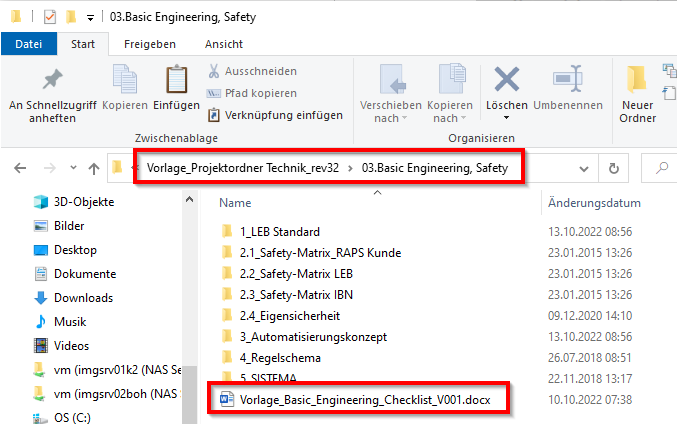
\includegraphics[width = 0.8 \textwidth]{Basic Engineering Checklist Ablageort.png}
    \caption{Basic Engineering Checklist Ablageort}
    \label{fig:Basic Engineering Checklist Ablageort}
\end{figure} 

\noindent \textbf{Diese Liste ist zu Beginn eines jeden Projektes durchzuarbeiten und auszufüllen!}

\clearpage
\section{Beispiele, warum Basic Engineering wichtig ist}\label{sec:Beispiele, warum Basic Engineering wichtig ist}

\subsection{1-kanaliger induktiver Sensor PLd -> besondere Beschaltung}\label[]{subsec:1-kanaliger induktiver Sensor PLd -> besondere Beschaltung}

Sensor: SICK IN40-D0303K

\begin{figure}[!ht]
    \centering
    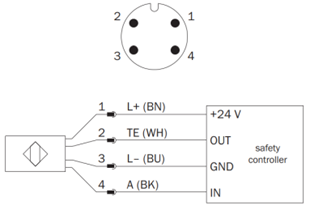
\includegraphics[width = 0.5 \textwidth]{SICK IN40 - D030K - Schaltbild.png}
    \caption{SICK IN40 - D030K - Schaltbild}
    \label{fig:SICK IN40 - D030K - Schaltbild}
\end{figure} 

\begin{figure}[!ht]
    \centering
    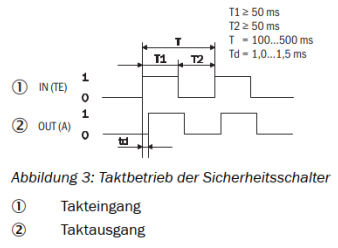
\includegraphics[width = 0.5 \textwidth]{SICK IN40-D0303K - Signalverhalten.png}
    \caption{SICK IN40-D0303K - Signalverhalten}
    \label{fig:SICK IN40-D0303K - Signalverhalten}
\end{figure}

\clearpage

\noindent Schaltungsbeispiel:

\begin{figure}[!ht]
    \centering
    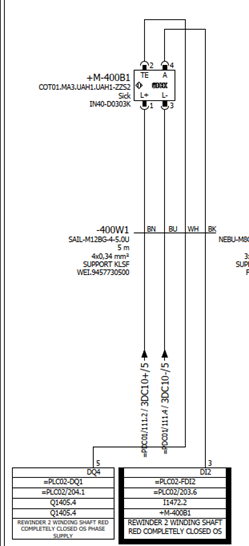
\includegraphics[width = 0.5 \textwidth]{Induktiver Sensor 1-kanalig PLd Schaltungsbeispiel.png}
    \caption{Induktiver Sensor 1-kanalig PLd Schaltungsbeispiel}
    \label{fig:Induktiver Sensor 1-kanalig PLd Schaltungsbeispiel}
\end{figure}

\noindent Um in 1-kanaliger Ausführung PLd zu erreichen, muss der Sensor selbst überwachen, dass eingangsseitig kein (Anschluss TE) kein Kurzschluss vorliegt. Daher ist auf dem Kanal ein gepulstes Signal vorzusehen, ansonsten geht der Sensor von einem Fehler aus und schaltet auch bei Betätigung nicht mehr.
Softwareseitig bietet Siemens dazu eine Lösung, die unter dem folgenden Link zu finden ist:

\noindent \url{https://support.industry.siemens.com/cs/document/109818998/sicheres-erfassen-mit-induktiver-taktender-sensorik-bis-sil-3-pl-d?dti=0&lc=de-DE} % \- for manual line break in url if necessary

\noindent Beitrags-ID SIOS: 109818998

\cite[\textbf{TODO!}]{todo}


\clearpage

\chapter{Projektcheckliste}\label{chap:Projektcheckliste}

    \begin{longtable}{| p{\colwidth{0.12}} | p{\colwidth{0.8}} | p{\colwidth{0.08}} |} % columns widths have to add up to 1 otherwise there will be an over- or underfill of the table layout
        \hline
        Typ & Punkt & OK \\
        \hline
        \endhead % save header to repeat it on each page          
        Projekt & Editiersprache und Referenzsprache korrekt eingestellt &  \\
        \hline      
        Projekt & \glqq Beim Übersetzen von Bausteinen Simulierbarkeit unterstützen\grqq{} aktiviert &  \\
        \hline      
        HW & SPS-Rechenleistung ausreichend &  \\
        \hline
        HW & SPS-Passwörter und Zugriffsschutz eingestellt &  \\
        \hline
        HW & SPS: Mehrsprachigkeit korrekt eingestellt &  \\
        \hline
        HW & SPS: F-Destination- und F-Source-Adressbereiche korrekt vergeben (Unter-/Obergrenze für F-Zieladressen, Zentrale F-Quelladresse) &  \\
        \hline
        HW & SPS Standard F-Überwachungszeit auf mindestens 300 ms &  \\
        \hline
        HW & Netzwerkteilnehmer Profisafe-Adressen Profisafe-Adresstyp \cite[\textbf{TODO!}]{todo} korrekt eingestellt(SPS-Adressbereiche beachten) &  \\
        \hline
        HW & An allen Netzwerkschnittstellen Default F-Überwachungszeit auf 300ms eingestellt &  \\
        \hline
        HW & Netzwerkteilnehmer vollständig angelegt (ET-Stationen, Antriebe, …) &  \\
        \hline
        HW & EA-Adressbereiche richtig eingestellt &  \\
        \hline
         & \cite[\textbf{TODO!}]{todo} &  \\
        \hline
        \caption{Projektcheckliste}\label{tab:Projektcheckliste} %\label used for referencing the figure in text
    \end{longtable}


\clearpage

\chapter{Einleitung}\label{chap:Einleitung}

\section{Leserkreis}\label{sec:Leserkreis}

Dieses Dokument ist für alle Mitarbeiter der Firma Lebbing engineering \& consulting GmbH der Abteilung Softwareengineering relevant.

\section{Literaturempfehlung}\label{sec:Literaturempfehlung}

Zum besseren Verständnis dieses Dokuments sei an dieser Stelle schon einmal auf die Dokumentation der Fa. Siemens zum TIA-Portal verwiesen, besonders wichtig sind dabei die Dokumente aus dem Kapitel 0.


\clearpage

\chapter{Wichtige Festlegungen}\label{chap:Wichtige Festlegungen}
\section{Platzhalter}\label{sec:Platzhalter}
Platzhalter werden in diesem Dokument dadurch symbolisiert, dass sie in spitzen Klammern gefasst sind, z.~B. <Platzhalter>. Optionale bzw. wiederholbare Platzhalter sind durch eckige Klammern $[~]$ und ggf. einen hoch- und/oder einen tiefgestellten Index n bzw. m versehen: $\nmsbracket{n}{m}{22}\mathrm{<Platzhalter>}]$. Die Indizes n und m kennzeichnen die maximale bzw. die minimale Anzahl für die Wiederholung des Platzhalters. Sollte der Index n nicht angegeben sein, darf der Platzhalter beliebig oft eingefügt werden. Falls der Index m nicht angegeben wurde, ist die Ausprägung des Platzhalters an der entsprechenden Stelle optional.


\clearpage

\input{6_Wichtige Erläuterungen Begriffsdefinitionen.tex}

\clearpage

\chapter{Grundeinstellungen TIA-Portal}\label{chap:Grundeinstellungen TIA-Portal}

\clearpage

\chapter{Projekterstellung}\label{chap:Projekterstellung}

\clearpage

\chapter{Hardwarekonfiguration}\label{chap:Hardwarekonfiguration}

\clearpage

\chapter{Regeln zur Softwareerstellung}\label{chap:Regeln zur Softwareerstellung}

\clearpage

\chapter{Antriebsprojektierung}\label{chap:Antriebsprojektierung}

\clearpage

\chapter{Visualisierung}\label{chap:Visualisierung}

\clearpage

\input{13_Mehrsprachigkeit Übersetzungen.tex}

\clearpage

\chapter{Funktionsbeschreibung}\label{chap:Funktionsbeschreibung}

\clearpage

\chapter{Multiuser}\label{chap:Multiuser}

\clearpage

\chapter{Inbetriebnahme}\label{chap:Inbetriebnahme}

\clearpage

\chapter{Troubleshooting}\label{chap:Troubleshooting}

\clearpage

\chapter{Beispielkapitel}\label{chap:example} % \label used for referencing the chapter in text

\lipsum[]

Das hier gezeigte \gls{latex}-Beispiel soll einige Möglichkeiten aufzeigen, wie ein Dokument gestaltet werden kann.

Das \acrfull{tia}-Portal ist eine Programmierumgebung, die speziell für die Projektierung von Siemens-Steuerungen entwickelt wurde. Im nachfolgenden wird die Abkürzung \acrshort{tia} aus Gründen der Lesbarkeit verwendet.

\begin{mycapequ}[!ht]
    \begin{equation}
        {P(\bigcup_{n=1}^n A_n) \leq \sum_{n=1}^n P(A_n)}
        \label{eq:bool} %\label used for referencing the equation in text
    \end{equation}
    \caption{Bool'sche Gleichung}
\end{mycapequ}

\noindent \cref{eq:bool} zeigt eine Gleichung in \gls{latex}.

\clearpage

\begin{figure}[!ht]
    \centering
    \includegraphics[width=1.0\textwidth]{example-image-a}
    \captionsetup{width=1.0\textwidth}
    \caption[skalierte Beispielabbildung]{skalierte Beispielabbildung (eigene Abbildung)}
    \label{fig:scaledexampleimagea} % \label used for referencing the figure in text
\end{figure}

\begin{figure}[!ht]
\centering
    \begin{minipage}[c]{.475\textwidth}
    \centering
        \includegraphics[width=1.0\linewidth]{example-image-b}
        \captionof{figure}[Beispielabbildung b]{Beispielabbildung b (eigene Abbildung)}
        \label{fig:horizontalalignedimageb} % \label used for referencing the figure in text
    \end{minipage}\hspace{.025\textwidth}
    \begin{minipage}[c]{.475\textwidth}
        \centering
        \includegraphics[width=1.0\linewidth]{example-image-c}
        \captionof{figure}[Beispielabbildung c]{Beispielabbildung c (eigene Abbildung)}
        \label{fig:horizontalalignedimagec} % \label used for referencing the figure in text
    \end{minipage}
\end{figure}

\noindent Oben sind einige Beispielabbildungen mit verschiedenen Skalierungen zu erkennen.

Außerdem besteht die Möglichkeit den Text, um ein Bild herum anzuordnen. Das sieht wie folgt aus.

\lipsum[1]

\begin{wrapfigure}{l}{0.4\textwidth}
    \centering
    \includegraphics[width=0.9\linewidth]{example-image}
    \captionsetup{width=0.9\linewidth}
    \caption[Beispielabbildung mit Text umrandet]{Beispielabbildung mit Text umrandet (eigene Abbildung)}
    \label{fig:textwrappedaroundexampleimage} % \label used for referencing the figure in text
\end{wrapfigure}

\lipsum[2-4]

\clearpage

\section{Beispielabschnitt}\label{sec:example} % \label used for referencing the section in text

\begin{table}[!ht]
    \centering
        \begin{tabular}{ | c | c | c | }
            \hline
            symbol & value & unit \\ \hline            
            $z Na$ & 11 & - \\ \hline      
            $z F$ & 9 & - \\ \hline      
            $Emax Na$ & 0.545 & $[MeV]$ \\ \hline
        \end{tabular}
        \caption{Beispieltabelle}
        \label{tab:example} % \label used for referencing the table in text
\end{table}

\noindent Hier (s.\cref{tab:example}) lässt sich eine kleine Beispieltabelle, die mit LaTeX erstellt wurde erkennen.

\clearpage

\section{Letzter Abschnitt}\label{sec:last} % \label used for referencing the section in text

\cref{fig:tikzexamplegraphics} zeigt eine Beispielgrafik, die mit dem Paket \glqq Tikz\grqq{} erstellt wurde.

\begin{figure}[!ht]
    \centering
	\begin{tikzpicture}
        \draw (0,0) circle (1);
        \draw (2,0) circle (1.5in);
        \draw (5,0) ellipse (10pt and 20 pt);
        \draw node at (3,0) {$f(x)$};
        \filldraw (6,0) circle (0.1cm) node[anchor=west]{Anchored Node};
    \end{tikzpicture}
    \caption{Tikz Beispielgrafik}
    \label{fig:tikzexamplegraphics} % \label used for referencing the figure in text
\end{figure}

\noindent Als ein weiteres komplexeres Beispiel kann hier auch noch folgende \cref{fig:tikzexamplediagram} angeführt werden.

\begin{figure}[!ht]
    \centering
    \begin{tikzpicture}[
                        youngnode/.style={rectangle, draw=red!60, fill=red!5, very thick, minimum size=40},
                        oldnode/.style={rectangle, draw=blue!60, fill=blue!5, very thick, minimum size=40},
                        ]
        %Nodes
        \node[oldnode]        (SusO)                            { $S_O(t)$};
        \node[oldnode]        (InfO)       [below=of SusO]      { $I_O(t)$};
        \node[oldnode]        (RecO)       [below=of InfO]      { $R_O(t)$};

        \node[youngnode]      (SusY)        [left=of SusO]      { $S_Y(t)$};
        \node[youngnode]      (InfY)        [left=of InfO]      { $I_Y(t)$};
        \node[youngnode]      (RecY)        [left=of RecO]      { $R_Y(t)$};

        %Lines
        \draw[->, very thick] (SusO.south east)  to node[right] {$a_{OO}$} (InfO.north east);
        \draw[->, very thick] (InfO.south)  to node[right] {$b_O$} (RecO.north);
        \draw[->, very thick] (RecO.east)  .. controls  +(right:17mm) and +(right:17mm)   .. (SusO.east);

        \draw[->, very thick] (SusY.south west)  to node[left] {$a_{YY}$} (InfY.north west);
        \draw[->, very thick] (InfY.south)  to node[left] {$b_Y$} (RecY.north);
        \draw[->, very thick] (RecY.west) .. controls  +(left:17mm) and +(left:17mm)   .. (SusY.west);

        \draw[dashed,->, very thick] (InfO.north west)  to  (SusY.south east);
        \draw[->, very thick] (SusY.south east)  to node[left] {$a_{OY}$} (InfY.north east);

        \draw[->, very thick] (SusO.south west)  to node[right] {$a_{YO}$} (InfO.north west);
        \draw[dashed,->, very thick] (InfY.north east)  to  (SusO.south west);
    \end{tikzpicture}
    \caption{Tikz Beispieldiagramm}
    \label{fig:tikzexamplediagram} % \label used for referencing the figure in text
\end{figure}

\clearpage

\noindent Das Paket \glqq pgfplots\grqq{} basiert auf \glqq Tikz\grqq{} und ermöglicht das Zeichnen von mathematischen Diagrammen aller Art. In \cref{fig:pgfplotsexample2D} ist dies anhand eines Beispiels dargestellt.

\begin{figure}[!ht]
    \centering
    \begin{tikzpicture}
        \begin{axis}[clip=false,xmin=0,xmax=2.5*pi,ymin=-1.5,ymax=1.5, axis lines=middle,xtick={0,pi/2,pi,3*pi/2,2*pi},xticklabels={$0$,$\frac{\pi}{2}$,$\pi$,$\frac{3}{2}\pi$,$2\pi$},xticklabel style={anchor=south west},xmajorgrids=true,grid style=dashed]
            \addplot[domain=0:2*pi,red]{sin(deg(x))}
            node[right,pos=0.9]{$f(x)=\sin x$};
            \addplot[domain=0:2*pi,blue]{cos(deg(x))}
            node[right,pos=1.0]{$g(x)=\cos x$};
        \end{axis}
    \end{tikzpicture}
    \caption{pgfplots Beispiel einer 2D-Grafik}
    \label{fig:pgfplotsexample2D} % \label used for referencing the figure in text
\end{figure}

\noindent Außerdem können auch 3D-Grafiken damit erstellt werden, wie in \cref{fig:pgfplotsexample3D} und in \cref{fig:anotherpgfplotsexample3D} zu sehen ist.

\begin{figure}[!ht]
    \centering
    \begin{tikzpicture}
        \begin{axis}[colormap/cool]
            \addplot3[mesh,samples=20]{1-x^2-y^2};
        \end{axis}
    \end{tikzpicture}
    \caption{pgfplots Beispiel einer 3D-Grafik}
    \label{fig:pgfplotsexample3D} % \label used for referencing the figure in text
\end{figure}

\clearpage

\begin{figure}[!ht]
    \centering
    \begin{tikzpicture}
        \begin{axis}[view={50}{30}]
            \addplot3+[domain=0:5*pi,samples=60,samples y=0]({sin(deg(x)},{cos(deg(x)},{x});
        \end{axis}
    \end{tikzpicture}
    \caption{weiteres pgfplots Beispiel einer 3D-Grafik}
    \label{fig:anotherpgfplotsexample3D} % \label used for referencing the figure in text
\end{figure}

\noindent Darüber hinaus können auch Daten aus .txt-Dateien ausgelesen werden und eine Grafik überführt werden (s. \cref{fig:pgfplotsexampledata}).

\begin{figure}[!ht]
    \centering
    \begin{minipage}[t]{1.0\linewidth}
        \centering
        \begin{tikzpicture}
            \begin{axis}[xmin=0, xmax=32, xlabel=$k$, ylabel=$x_k$, ymin=0, ymax=1, ymajorgrids=true, xmajorgrids=true, width=0.95\linewidth]
                \addplot+[only marks] table[x=k, y=hk]{data/exampledata.txt};
            \end{axis}
        \end{tikzpicture}
        \caption{Beispiel einer Datenreihe mit pgfplot}
        \label{fig:pgfplotsexampledata} % \label used for referencing the figure in text
    \end{minipage}
\end{figure}

\noindent Weitere Informationen zu den Paketen gibt es in der Dokumentation unter \cite{tikz} und \cite{pgfplots}.

\clearpage

% --- bibliography --- %

\pagenumbering{Roman}
\setcounter{page}{\thesavepage}

\printbibliography[heading = bibintoc,
                   title = Literaturverzeichnis]

\clearpage

%---- appendix ----%

\appendix

\chapter{Anhang}\label{chap:Anhang}

\clearpage

%---- glossary ----%

\printnoidxglossary[style=long, title={Glossar}]

\clearpage

\end{document}
